\documentclass[border=20pt, preview]{standalone}
\usepackage[american]{circuitikz}
\usepackage{amsmath}% To allow \cfrac macro
\usepackage{bm}% Bold math
\usetikzlibrary{arrows.meta,decorations.markings}

\begin{document}
  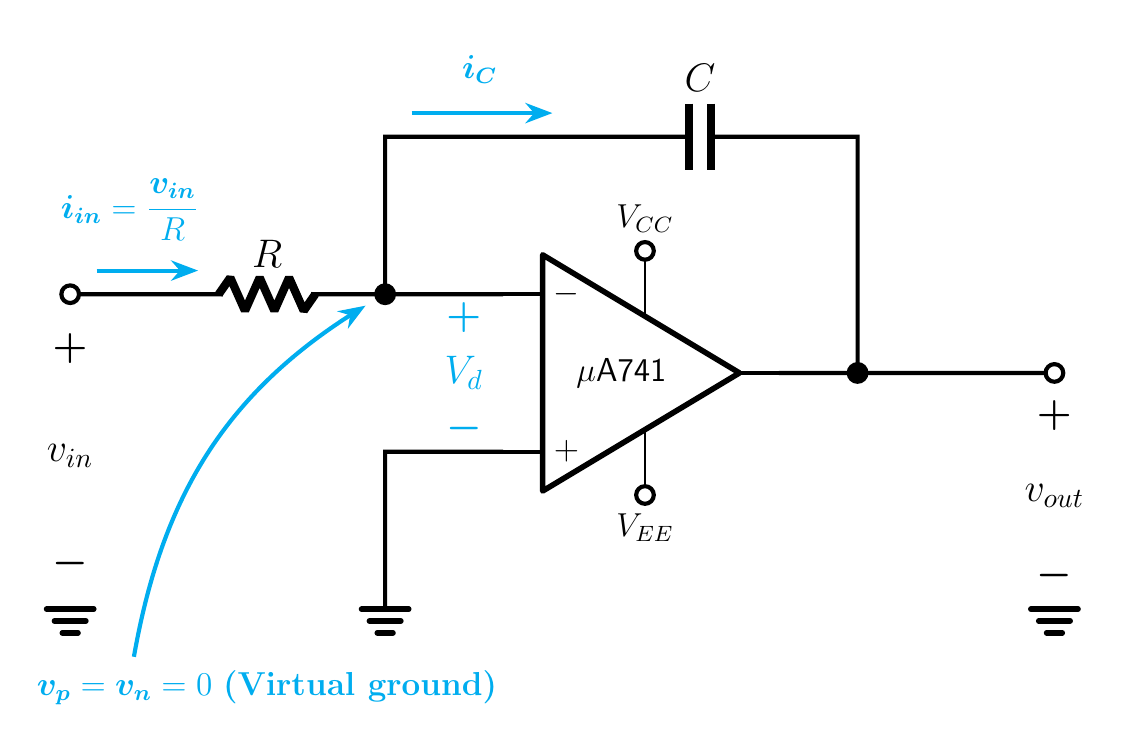
\begin{tikzpicture}[
    % Environment Config
    font=\large,
    MyArrow/.style={% Style for the current
      -Stealth,
      cyan,
      line width=1.5pt,
      shorten >= 5pt,
      shorten <= 1pt
    },
    Vref/.style={% Style for the voltage reference
      draw=none,
      postaction={decorate,decoration={markings,mark=at position 0.5 with {\node{\Large #1};}}},
      postaction={decorate,decoration={markings,mark=at position 0.15 with {\node{\Large $\bm{+}$};}}},
      postaction={decorate,decoration={markings,mark=at position 0.85 with {\node{\Large $\bm{-}$};}}}
    },
    Numbered/.style = {% Style for circle marks
      draw,
      circle,
      line width=1.5pt,
      align=center,
      inner sep=4pt,
      label distance=15pt
    }
  ]

  \def\MyOpamp(#1)#2{% Custom opamp
    \begin{scope}[shift={(#1)}]
      %===Component Shape===
      \draw[line width = 2pt, line join=round] (0,0)++(-1,1.5)
        --++(2.5,-1.5) -- ++(-2.5,-1.5)-- cycle;
      %===Label===
      \draw(0,0) node{\sf $\mu$A741};
      %===PIN: IN-===
      \draw[line width = 1.5pt] (-1,1) node [anchor=180]{$-$} -- ++(-0.5,0)  coordinate (#2 IN-);
      %===PIN: N+===
      \draw[line width = 1.5pt] (-1,-1) node [anchor=180]{$+$}  -- ++(-0.5,0) coordinate (#2 IN+);
      %===PIN: OUT===
      \draw[line width = 1.5pt] (1.5,0)  -- ++(0.5,0) coordinate (#2 OUT);
      %===PIN: Vcc===
      \draw[line width = 1pt] (0.3, 0.75) -- ++(0, 0.8) coordinate (#2 Vcc);
      \draw(0.3,1.55) node[ocirc,scale=2,line width=1.5pt, label=above:$V_{CC}$]{};
      %===PIN: Vee===
      \draw[line width = 1pt] (0.3, -0.75) -- ++(0, -0.8) coordinate (#2 Vee);
      \draw(0.3,-1.55) node[ocirc,scale=2,line width=1.5pt, label=below:$V_{EE}$]{};
    \end{scope}
  }
  \def\MyGround(#1)#2{% Customized Ground
    \begin{scope}[shift={(#1)}]
      % Component Shape
      \draw[line width = 2pt, line cap=round]
      (0,0) coordinate (#2 GND)++(-0.3,0)--++(0.6,0)
      (0,-0.15)++(-0.2,0)--++(0.4,0)
      (0,-0.3)++(-0.1,0)--++(0.2,0);
    \end{scope}
  }

  % Put the customzed opamp in position
  \MyOpamp(0,0){1}

  % Put some short nodes
  \draw(-7,1) node[ocirc,scale=2,line width=1.5pt](N3){};
  \draw(-3,1) node[circ,scale=2,line width=1.5pt](N2){};
  \draw(3,0) node[circ,scale=2,line width=1.5pt](N6){};
  \draw(5.5,0) node[ocirc,scale=2,line width=1.5pt](N6-OUT){};
  \MyGround(-7,-3){1}
  \MyGround(1 GND -| N2){2}
  \MyGround(1 GND -| N6-OUT){3}

  % Draw the Wires and pasive components
  \draw[line width=1.5pt]
  (N3)%From node N3
      --++(1,0)
      to [R,l=\Large$R$] (N2)
      --(1 IN-)
  (N2)
      --++(0,2) coordinate (N5)
      --++(2.5,0)
      to[C,l=\Large$C$]++(3,0)
      -| (N6)
  (1 OUT)
      -- (N6-OUT)
  (1 IN+)
      -|(2 GND);

  % Voltage references
  %===Vin===
  \draw[Vref=$v_{in}$]
  (N3)
      -- (1 GND);

  %===Vd===
  \draw[Vref=$V_d$,color=cyan]
  (1 IN-)
      ++(-0.5,0) coordinate (temp)
      -- (1 IN+ -| temp)
      node[
          midway,
      ]{};

  %===Vout===
  \draw[Vref=$v_{out}$]
  (N6-OUT)
      -- (3 GND);
      % ===Equation:Vout===
      % node [
      %     midway,
      %     % label={[Numbered,black,label distance=5pt]180:\bf 6}
      % ]{$\bm{v_{out}}$};

  %===Virtual Ground===
  \draw[MyArrow]
  (N2)++(-1.5,-5)
      node [](C1){$\bm{v_p} = \bm{v_n} = 0$ \bf (Virtual ground)}
  (C1.168) %get a point from center to node box at 168 degrees
      to [out=80, in=-150] (N2);

  % Draw currents
  %===Iin===
  \draw[MyArrow]
  (N3)++(0.3,0.3)
      -- ++(1.5,0)
      node [
          midway,
          inner sep=10pt,
          anchor=-70,
          % label={[Numbered,black,label distance=0pt]180:\bf 3}
      ]{$\bm{i_{in}} = \cfrac{\bm{v_{in}}}{R}$};

  %===Ic===
  \draw[MyArrow]
  (N5)++(0.3,0.3) %node gap
      -- ++(2,0) % Arrow longitude
      node [
          midway,
          inner sep=10pt,
          anchor=-80,
          % label={[Numbered,black,label distance=0pt]180:\bf 5}
      ]{$\bm{i_C}$};

  \end{tikzpicture}
\end{document}